\section{Senior Project Overview}

In 2014, Erik Brunvand proposed the idea of constructing an ASIC tester using an FPGA and a digital clock manager. Daniel immediately took interest in the idea and later formed a team with Norm Gifford, Tyler Martinsen, and Ruben Gottardi. This section glosses over our senior project to provide context of where the ideas for our Master's project stem from. Detailed information about our senior project can be found on our repository. 

\subsection{Project Architecture}

\subsubsection{Hardware Flow}
Figure \ref{fig:senior_project_hardware_flow} illustrates the four hardware components of their board: 
\begin{itemize}
\item A \textbf{PC} provides a program for user-interfacing. Written in C Sharp, this program first reads and parses a text file that configures the tester. (This text file is largely based upon the .msa file format used by the LV500.) Through a serial connection, the PC then transmits the contents of the text file to a Xilinx \textbf{MicroBlaze} processor running on a \textbf{Digilent Atlys board}. 
\item The \textbf{MicroBlaze} processor simply converts the serial commands retrieved from the PC into SPI commands suited for the \textbf{Numato Saturn Spartan-6 FPGA board}.
\item The \textbf{Numato Saturn} houses the logic that is used to execute a single test cycle. In particular, the FPGA sends signals to the DUT on the \textbf{main PCB} and samples output signals from the DUT. 
\item The \textbf{main PCB} simply contains 139 voltage translators and a ZIF socket to house the DUT. 
\end{itemize}

\begin{figure}
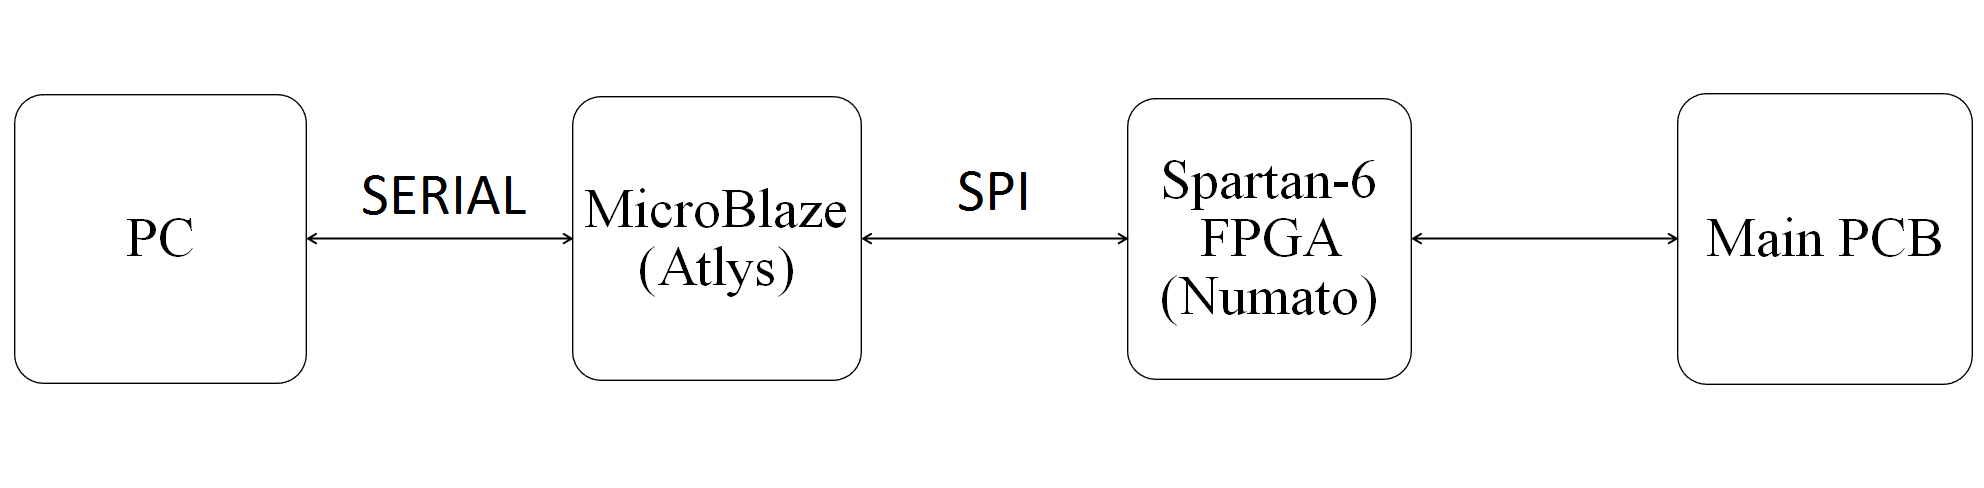
\includegraphics[width=1.0\textwidth]{senior_project_hardware_flow_diagram.png}
\caption{Senior project hardware flow diagram.}
\label{fig:senior_project_hardware_flow}
\end{figure}

\subsubsection{Software Flow}

Figure \ref{fig:senior_project_software_flow} illustrates the flow of the C Sharp program used to interface with the tester. The key observation is that the C Sharp program parses and transmits to the MicroBlaze processor a \textbf{single} input vector at a time. For every input vector parsed, that input vector makes its way to the Numato Saturn, which executes that test vector and samples the outputs of the DUT. The C Sharp program then sends a request to the MicroBlaze processor, asking for the output vector stored in the FPGA. After retrieving the output vector and comparing the sampled bits to the bits expected by the user, the C Sharp program parses and transmits the next input vector. When all input vectors are processed, the results are displayed to the user.

\begin{figure}
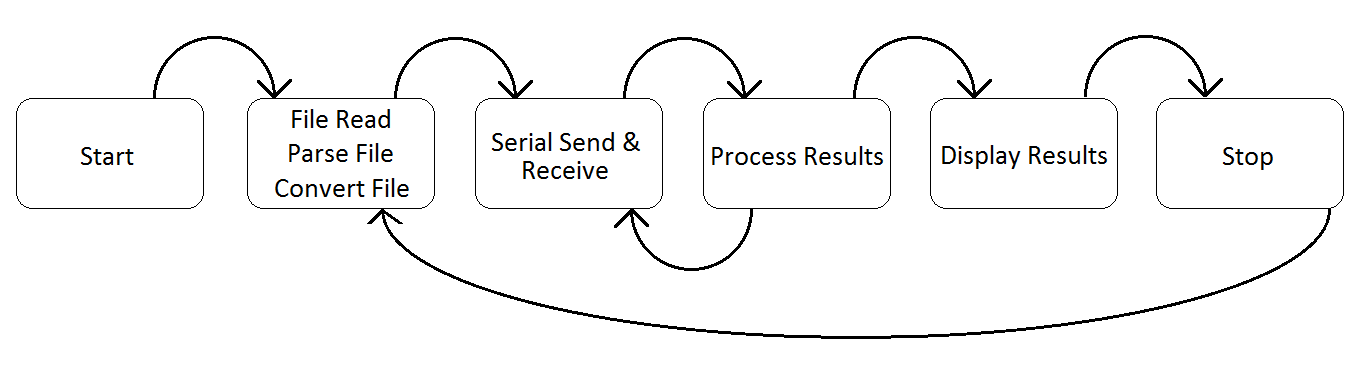
\includegraphics[width=1.0\textwidth]{senior_project_software_flow_diagram.png}
\caption{Senior project hardware flow diagram.}
\label{fig:senior_project_software_flow}
\end{figure}

\subsection{What Worked}
There are three features of our system that we excelled in: 
\begin{itemize}
\item \textbf{Functional testing} appeared to work fine. Our system was able to correctly test circuits like an inverter, AND gate, OR gate, and DFF. (A note: We define functional testing as simply seeing if the outputs of a DUT respond correctly to the inputs applied to the DUT, with no timing or electrical characteristics of the DUT taken into account.)
\item Unlike the LV500, our system \textbf{does not contain fixed VDD and GND locations} for the DUT. VDD and GND are provided to the DUT using jumper wires and jumper pins. 
\item \textbf{Manual schooming} was enabled using a variable voltage regulator and separate power jacks for the DUT VDD and FPGA VDD.
\end{itemize}

\subsection{Areas of Improvement}
Although functional testing - the key feature of our system - appeared to work, there were several areas of improvement that prevented our project from serving as a substitute for the LV500 and Verigy 93000 testers: 
\begin{itemize}
\item Since every input vector must travel through the entire hardware pipeline and back, \textbf{real-time testing}, which we define as executing a test cycle immediately after the completion of a preceding test cycle, is not possible with the design that we chose. Real-time testing can help provide more detailed timing information about a DUT.
\item \textbf{Autoschmooing}, which we define as schmooing controlled by the hardware/software, is not supported. Obviously, autoschmooing is far more convenient than manual schmooing, and autoschmooing allows the system to generate plots of when the DUT's output vectors match expectations and when they don't.
\item Our system only supports \textbf{one template}, due to lack of time. Multiple templates are needed for any chips with bidirectional pins.
\item The MicroBlaze processor had to be reprogrammed everytime power was cut off from the Atlys board. This issue, along with the inclusion of the Atlys board itself, made the system as a whole \textbf{clumsy and unintuitive to use}. (A note: We intended to program MicroBlaze onto the Numato Saturn but had difficulties doing so.)
\item We attempted to utilize a PLL package provided by Xilinx to allow dynamically-reconfigurable frequencies, phase shifts, and duty cycles for the internal test cycles (i.e. the clock waveforms that represent the length, width, and delay of a test cycle). The PLL proved to be problematic, however; the best performance we obtained was from fixing the frequencies of the PLL's outputs at 2 MHz and offering just a few options for phase shifts and duty cycles. Having \textbf{highly configurable} test cycles is crucial to obtain timing information about a chip.
\item  Because our main PCB board lacked equilibrium tracing, we were unable to provide a \textbf{reasonable average for the wire delay} between the DUT and FPGA, which again impeded our ability to provide timing information of the DUT to the user.
\end{itemize}

\newpage